\documentclass[]{book}
\usepackage{lmodern}
\usepackage{amssymb,amsmath}
\usepackage{ifxetex,ifluatex}
\usepackage{fixltx2e} % provides \textsubscript
\ifnum 0\ifxetex 1\fi\ifluatex 1\fi=0 % if pdftex
  \usepackage[T1]{fontenc}
  \usepackage[utf8]{inputenc}
\else % if luatex or xelatex
  \ifxetex
    \usepackage{mathspec}
  \else
    \usepackage{fontspec}
  \fi
  \defaultfontfeatures{Ligatures=TeX,Scale=MatchLowercase}
\fi
% use upquote if available, for straight quotes in verbatim environments
\IfFileExists{upquote.sty}{\usepackage{upquote}}{}
% use microtype if available
\IfFileExists{microtype.sty}{%
\usepackage{microtype}
\UseMicrotypeSet[protrusion]{basicmath} % disable protrusion for tt fonts
}{}
\usepackage[margin=1in]{geometry}
\usepackage{hyperref}
\hypersetup{unicode=true,
            pdftitle={Automated Gating of Flow Cytometry Data using the Bioconductor openCyto Framework},
            pdfauthor={Nichole Monhait, MPH Candidate; Colorado School of Public Health, Colorado State University},
            pdfborder={0 0 0},
            breaklinks=true}
\urlstyle{same}  % don't use monospace font for urls
\usepackage{natbib}
\bibliographystyle{plainnat}
\usepackage{color}
\usepackage{fancyvrb}
\newcommand{\VerbBar}{|}
\newcommand{\VERB}{\Verb[commandchars=\\\{\}]}
\DefineVerbatimEnvironment{Highlighting}{Verbatim}{commandchars=\\\{\}}
% Add ',fontsize=\small' for more characters per line
\usepackage{framed}
\definecolor{shadecolor}{RGB}{248,248,248}
\newenvironment{Shaded}{\begin{snugshade}}{\end{snugshade}}
\newcommand{\AlertTok}[1]{\textcolor[rgb]{0.94,0.16,0.16}{#1}}
\newcommand{\AnnotationTok}[1]{\textcolor[rgb]{0.56,0.35,0.01}{\textbf{\textit{#1}}}}
\newcommand{\AttributeTok}[1]{\textcolor[rgb]{0.77,0.63,0.00}{#1}}
\newcommand{\BaseNTok}[1]{\textcolor[rgb]{0.00,0.00,0.81}{#1}}
\newcommand{\BuiltInTok}[1]{#1}
\newcommand{\CharTok}[1]{\textcolor[rgb]{0.31,0.60,0.02}{#1}}
\newcommand{\CommentTok}[1]{\textcolor[rgb]{0.56,0.35,0.01}{\textit{#1}}}
\newcommand{\CommentVarTok}[1]{\textcolor[rgb]{0.56,0.35,0.01}{\textbf{\textit{#1}}}}
\newcommand{\ConstantTok}[1]{\textcolor[rgb]{0.00,0.00,0.00}{#1}}
\newcommand{\ControlFlowTok}[1]{\textcolor[rgb]{0.13,0.29,0.53}{\textbf{#1}}}
\newcommand{\DataTypeTok}[1]{\textcolor[rgb]{0.13,0.29,0.53}{#1}}
\newcommand{\DecValTok}[1]{\textcolor[rgb]{0.00,0.00,0.81}{#1}}
\newcommand{\DocumentationTok}[1]{\textcolor[rgb]{0.56,0.35,0.01}{\textbf{\textit{#1}}}}
\newcommand{\ErrorTok}[1]{\textcolor[rgb]{0.64,0.00,0.00}{\textbf{#1}}}
\newcommand{\ExtensionTok}[1]{#1}
\newcommand{\FloatTok}[1]{\textcolor[rgb]{0.00,0.00,0.81}{#1}}
\newcommand{\FunctionTok}[1]{\textcolor[rgb]{0.00,0.00,0.00}{#1}}
\newcommand{\ImportTok}[1]{#1}
\newcommand{\InformationTok}[1]{\textcolor[rgb]{0.56,0.35,0.01}{\textbf{\textit{#1}}}}
\newcommand{\KeywordTok}[1]{\textcolor[rgb]{0.13,0.29,0.53}{\textbf{#1}}}
\newcommand{\NormalTok}[1]{#1}
\newcommand{\OperatorTok}[1]{\textcolor[rgb]{0.81,0.36,0.00}{\textbf{#1}}}
\newcommand{\OtherTok}[1]{\textcolor[rgb]{0.56,0.35,0.01}{#1}}
\newcommand{\PreprocessorTok}[1]{\textcolor[rgb]{0.56,0.35,0.01}{\textit{#1}}}
\newcommand{\RegionMarkerTok}[1]{#1}
\newcommand{\SpecialCharTok}[1]{\textcolor[rgb]{0.00,0.00,0.00}{#1}}
\newcommand{\SpecialStringTok}[1]{\textcolor[rgb]{0.31,0.60,0.02}{#1}}
\newcommand{\StringTok}[1]{\textcolor[rgb]{0.31,0.60,0.02}{#1}}
\newcommand{\VariableTok}[1]{\textcolor[rgb]{0.00,0.00,0.00}{#1}}
\newcommand{\VerbatimStringTok}[1]{\textcolor[rgb]{0.31,0.60,0.02}{#1}}
\newcommand{\WarningTok}[1]{\textcolor[rgb]{0.56,0.35,0.01}{\textbf{\textit{#1}}}}
\usepackage{longtable,booktabs}
\usepackage{graphicx,grffile}
\makeatletter
\def\maxwidth{\ifdim\Gin@nat@width>\linewidth\linewidth\else\Gin@nat@width\fi}
\def\maxheight{\ifdim\Gin@nat@height>\textheight\textheight\else\Gin@nat@height\fi}
\makeatother
% Scale images if necessary, so that they will not overflow the page
% margins by default, and it is still possible to overwrite the defaults
% using explicit options in \includegraphics[width, height, ...]{}
\setkeys{Gin}{width=\maxwidth,height=\maxheight,keepaspectratio}
\IfFileExists{parskip.sty}{%
\usepackage{parskip}
}{% else
\setlength{\parindent}{0pt}
\setlength{\parskip}{6pt plus 2pt minus 1pt}
}
\setlength{\emergencystretch}{3em}  % prevent overfull lines
\providecommand{\tightlist}{%
  \setlength{\itemsep}{0pt}\setlength{\parskip}{0pt}}
\setcounter{secnumdepth}{5}
% Redefines (sub)paragraphs to behave more like sections
\ifx\paragraph\undefined\else
\let\oldparagraph\paragraph
\renewcommand{\paragraph}[1]{\oldparagraph{#1}\mbox{}}
\fi
\ifx\subparagraph\undefined\else
\let\oldsubparagraph\subparagraph
\renewcommand{\subparagraph}[1]{\oldsubparagraph{#1}\mbox{}}
\fi

%%% Use protect on footnotes to avoid problems with footnotes in titles
\let\rmarkdownfootnote\footnote%
\def\footnote{\protect\rmarkdownfootnote}

%%% Change title format to be more compact
\usepackage{titling}

% Create subtitle command for use in maketitle
\newcommand{\subtitle}[1]{
  \posttitle{
    \begin{center}\large#1\end{center}
    }
}

\setlength{\droptitle}{-2em}

  \title{Automated Gating of Flow Cytometry Data using the Bioconductor \texttt{openCyto} Framework}
    \pretitle{\vspace{\droptitle}\centering\huge}
  \posttitle{\par}
    \author{Nichole Monhait, MPH Candidate \\ Colorado School of Public Health, Colorado State University}
    \preauthor{\centering\large\emph}
  \postauthor{\par}
      \predate{\centering\large\emph}
  \postdate{\par}
    \date{2019-05-01}

\usepackage{booktabs}

\begin{document}
\maketitle

{
\setcounter{tocdepth}{1}
\tableofcontents
}
\hypertarget{whats-inside}{%
\chapter{What's inside?}\label{whats-inside}}

The goal of this tutorial is to take manually gated data from a .wsp flowJo file and use the Bioconductor \texttt{openCyto} framework to create an automated gating procedure within R which can be replicated on any dataset. The basic functions used in this tutorial include:

\emph{openWorkspace()\\
}parseWorkspace()\\
\emph{gatingTemplate()\\
}gating()\\
\emph{plot()\\
}plotGate()

The example data used in this tutorial is from Colorado State University's Microbiology, Immunology, and Pathology Department. Alternatively, you can input your own flowJo Workspace and follow this tutorial, so long as the file is in .wsp format.

\hypertarget{getting-started}{%
\chapter{Getting Started}\label{getting-started}}

Here is an overview of the process to automate flow cytometry data using R's \texttt{openCyto} and what you will need to successfully automate your own flow cytometry analysis. The general steps to accomplish this are as follows:

\begin{enumerate}
\def\labelenumi{\arabic{enumi}.}
\tightlist
\item
  Read in a manually gated flowJo workspace in .wsp file format.
\item
  Parse raw FCS files from the read in workspace.
\item
  Visualize the manual gating template and resulting gates to verify gating scheme.
\item
  Create and read in a .csv gating template.
\item
  Automate gating.
\item
  Visualize automated gating template and gates to verify gating scheme.
\item
  Extract population statistics and relevant information.
\end{enumerate}

This process is completed primarily with the \texttt{openCyto} package but calls upon other packages within the Bioconductor \texttt{openCyto} framework. Packages needed to complete this tutorial are listed at the end of this chapter. Descriptions of each function and R object used for this analysis are below.

\hypertarget{function-and-r-object-definitions}{%
\section{Function and R Object Definitions}\label{function-and-r-object-definitions}}

\begin{tabular}{c|c}
\hline
Function/Object Name & Definition\\
\hline
wsfile & flowJo .wsp file location\\
\hline
openWorkspace() & function used to read in **wsfile**\\
\hline
ws & read in data from flowJo\\
\hline
parseWorkspace() & function to extract FCS files from **ws**\\
\hline
gating\_set & parsed FCS files to be gated\\
\hline
clone() & function used to create a clone of **gating\_set**\\
\hline
gh & subset of gating\_set\\
\hline
gt & .csv gating template\\
\hline
templateGen() & function used to generate a .csv template from existing manual gates\\
\hline
gatingTemplate() & function used to read in .csv template\\
\hline
gating() & function used to apply gates to a gating set\\
\hline
plot() & function to visualize gating tree\\
\hline
plotGate() & function to visualize gates\\
\hline
\end{tabular}

\hypertarget{required-packages-and-installation}{%
\section{Required Packages and Installation}\label{required-packages-and-installation}}

Before getting started, install and load the following libraries into a new R script. As you will see below, this tutorial uses the development version of \texttt{openCyto}. Use the following to ensure the correct packages are installed.

\emph{To install}

\begin{Shaded}
\begin{Highlighting}[]
\NormalTok{devtools}\OperatorTok{::}\KeywordTok{install_github}\NormalTok{(}\StringTok{"RGLab/openCyto"}\NormalTok{, }\DataTypeTok{ref =} \StringTok{"trunk"}\NormalTok{)}
\KeywordTok{install.packages}\NormalTok{(}\StringTok{"data.table"}\NormalTok{)}
\KeywordTok{install.packages}\NormalTok{(}\StringTok{"flowWorkspace"}\NormalTok{)}
\KeywordTok{install.packages}\NormalTok{(}\StringTok{"flowCore"}\NormalTok{)}
\KeywordTok{install.packages}\NormalTok{(}\StringTok{"flowStats"}\NormalTok{)}
\KeywordTok{install.packages}\NormalTok{(}\StringTok{"flowClust"}\NormalTok{)}
\KeywordTok{install.packages}\NormalTok{(}\StringTok{"plyr"}\NormalTok{)}
\end{Highlighting}
\end{Shaded}

\emph{To load}

\begin{Shaded}
\begin{Highlighting}[]
\KeywordTok{library}\NormalTok{(openCyto)}
\KeywordTok{library}\NormalTok{(flowWorkspace)}
\KeywordTok{library}\NormalTok{(data.table)}
\KeywordTok{library}\NormalTok{(flowCore)}
\KeywordTok{library}\NormalTok{(flowStats)}
\KeywordTok{library}\NormalTok{(flowClust)}
\KeywordTok{library}\NormalTok{(plyr)}
\end{Highlighting}
\end{Shaded}

\hypertarget{working-with-your-manual-gating-scheme}{%
\chapter{Working with your Manual Gating Scheme}\label{working-with-your-manual-gating-scheme}}

Current methods for manually gating flow cytometry are both time consuming and costly, making automated gating an appealing option. The \texttt{openCyto} package allows users to take manually gated data from flowJo, reproduce those gates in R, and eventually automate the gating process.

The first step in this process is to bring a pre-existing flowJo file into R in order to recreate the gating environment. The remainder of this chapter will detail the following:

\begin{enumerate}
\def\labelenumi{\arabic{enumi}.}
\tightlist
\item
  Read in flowJo .wsp file\\
\item
  Parse FCS files\\
\item
  Visualize and verify manual gates
\item
  Clone data for later automation
\end{enumerate}

\hypertarget{read-in-flowjo-file}{%
\section{Read in flowJo file}\label{read-in-flowjo-file}}

Within flowJo, tranformation, compensation, and gating can be saved as either .xml or .wsp filetypes. This tutorial will only detail steps from a \emph{.wsp} filetype saved from flowJo. Saving analysis within flowJo is detailed \href{http://docs.flowjo.com/vx/workspaces-and-samples/ws-savinganalysis/}{here}.

The result of step 1 will be replication of the manual transformation, compensation, and gating from the flowJo workspace saved as an R object. Before you begin, be sure you have loaded the required packages outlined in the previous chapter.

Once all packages are loaded, save the .wsp file path as an R object called \textbf{wsfile}. Next, use \texttt{openWorkspace()} with your R object name to open the .wsp file in R, save this as \textbf{ws}. Here is an example of saving and opening \textbf{wsfile}. Following this step, \textbf{ws} will be saved as a flowWorkspace object containing groups of samples.

\begin{Shaded}
\begin{Highlighting}[]
\KeywordTok{library}\NormalTok{(openCyto)}
\KeywordTok{library}\NormalTok{(flowWorkspace)}
\KeywordTok{library}\NormalTok{(data.table)}
\KeywordTok{library}\NormalTok{(flowCore)}
\KeywordTok{library}\NormalTok{(flowStats)}
\KeywordTok{library}\NormalTok{(flowClust)}
\KeywordTok{library}\NormalTok{(plyr)}
\end{Highlighting}
\end{Shaded}

\begin{Shaded}
\begin{Highlighting}[]
\NormalTok{wsfile <-}\StringTok{ "/Users/monhait/Desktop/flow_cyto/automated_gating/data/Young_v_Adult_D30_Tcell_Spleen.wsp"}
\end{Highlighting}
\end{Shaded}

\begin{Shaded}
\begin{Highlighting}[]
\NormalTok{ws <-}\StringTok{ }\KeywordTok{openWorkspace}\NormalTok{(wsfile)}
\end{Highlighting}
\end{Shaded}

\begin{Shaded}
\begin{Highlighting}[]
\KeywordTok{print}\NormalTok{(ws)}
\end{Highlighting}
\end{Shaded}

\begin{verbatim}
## FlowJo Workspace Version  20.0 
## File location:  /Users/monhait/Desktop/flow_cyto/automated_gating/data 
## File name:  Young_v_Adult_D30_Tcell_Spleen.wsp 
## Workspace is open. 
## 
## Groups in Workspace
##          Name Num.Samples
## 1 All Samples          10
## 2     Samples          10
\end{verbatim}

\hypertarget{parse-fcs-files}{%
\section{Parse FCS files}\label{parse-fcs-files}}

Once this file exists as an R object, the raw FCS files are then read using the \texttt{parseWorkspace} function. This function will read the FCS files and transform, compensate, and gate according to parameters defined from the .wsp flowJo workspace. The \texttt{parseWorskpace} call requires \textbf{ws} (the .wsp workspace that was just read in from flowJo) and the name of the samples to read in. Other options may be customized based on particular needs. A new R object named \textbf{gating\_set} is then created and will be a GatingSet object. The \textbf{isNcdf = TRUE} call saves this output to disk rather that into memory because the files are large. Here is an example of parsing FCS files.

\begin{Shaded}
\begin{Highlighting}[]
\NormalTok{gating_set <-}\StringTok{ }\KeywordTok{parseWorkspace}\NormalTok{(ws, }\DataTypeTok{name =} \StringTok{"Samples"}\NormalTok{, }\DataTypeTok{path =} \StringTok{"/Users/monhait/Desktop/flow_cyto/automated_gating/data/fcs"}\NormalTok{, }\DataTypeTok{isNcdf =} \OtherTok{TRUE}\NormalTok{, }\DataTypeTok{sampNloc =} \StringTok{'sampleNode'}\NormalTok{)}
\end{Highlighting}
\end{Shaded}

\begin{verbatim}
## Parsing 10 samples
\end{verbatim}

\begin{verbatim}
## windows version of flowJo workspace recognized.
## version X
\end{verbatim}

\begin{verbatim}
## Creating ncdfFlowSet...
\end{verbatim}

\begin{verbatim}
## All FCS files have the same following channels:
## Time
## SSC-H
## SSC-A
## FSC-H
## FSC-A
## BV421-H
## BV480-H
## BV510-H
## BV570-H
## BV605-H
## BV650-H
## BV711-H
## BV785-H
## BB515-H
## Alexa Fluor 532-H
## PE-H
## PE-Dazzle594-H
## PE-Cy5-H
## PerCP-Cy5.5-H
## PerCP-eFluor 710-H
## PE-Cy7-H
## APC-H
## APC-R700-H
## APC-Fire 750-H
## Zombie Nir-H
## AF-H
## BV421-A
## BV480-A
## BV510-A
## BV570-A
## BV605-A
## BV650-A
## BV711-A
## BV785-A
## BB515-A
## Alexa Fluor 532-A
## PE-A
## PE-Dazzle594-A
## PE-Cy5-A
## PerCP-Cy5.5-A
## PerCP-eFluor 710-A
## PE-Cy7-A
## APC-A
## APC-R700-A
## APC-Fire 750-A
## Zombie Nir-A
## AF-A
\end{verbatim}

\begin{verbatim}
## done!
\end{verbatim}

\begin{verbatim}
## loading data: /Users/monhait/Desktop/flow_cyto/automated_gating/data/fcs/SPLEEN_ADULT 1_20180823_174115_Unmixed.fcs
\end{verbatim}

\begin{verbatim}
## Compensating
\end{verbatim}

\begin{verbatim}
## gating ...
\end{verbatim}

\begin{verbatim}
## write SPLEEN_ADULT 1_20180823_174115_Unmixed.fcs_142158 to empty cdf slot...
\end{verbatim}

\begin{verbatim}
## loading data: /Users/monhait/Desktop/flow_cyto/automated_gating/data/fcs/SPLEEN_ADULT 2_20180823_174227_Unmixed.fcs
\end{verbatim}

\begin{verbatim}
## Compensating
\end{verbatim}

\begin{verbatim}
## gating ...
\end{verbatim}

\begin{verbatim}
## write SPLEEN_ADULT 2_20180823_174227_Unmixed.fcs_130445 to empty cdf slot...
\end{verbatim}

\begin{verbatim}
## loading data: /Users/monhait/Desktop/flow_cyto/automated_gating/data/fcs/SPLEEN_ADULT 3_20180823_174339_Unmixed.fcs
\end{verbatim}

\begin{verbatim}
## Compensating
\end{verbatim}

\begin{verbatim}
## gating ...
\end{verbatim}

\begin{verbatim}
## write SPLEEN_ADULT 3_20180823_174339_Unmixed.fcs_140448 to empty cdf slot...
\end{verbatim}

\begin{verbatim}
## loading data: /Users/monhait/Desktop/flow_cyto/automated_gating/data/fcs/SPLEEN_ADULT 4_20180823_174455_Unmixed.fcs
\end{verbatim}

\begin{verbatim}
## Compensating
\end{verbatim}

\begin{verbatim}
## gating ...
\end{verbatim}

\begin{verbatim}
## write SPLEEN_ADULT 4_20180823_174455_Unmixed.fcs_131634 to empty cdf slot...
\end{verbatim}

\begin{verbatim}
## loading data: /Users/monhait/Desktop/flow_cyto/automated_gating/data/fcs/SPLEEN_ADULT 5_20180823_174556_Unmixed.fcs
\end{verbatim}

\begin{verbatim}
## Compensating
\end{verbatim}

\begin{verbatim}
## gating ...
\end{verbatim}

\begin{verbatim}
## write SPLEEN_ADULT 5_20180823_174556_Unmixed.fcs_127923 to empty cdf slot...
\end{verbatim}

\begin{verbatim}
## loading data: /Users/monhait/Desktop/flow_cyto/automated_gating/data/fcs/SPLEEN_YOUNG 1_20180823_173545_Unmixed.fcs
\end{verbatim}

\begin{verbatim}
## Compensating
\end{verbatim}

\begin{verbatim}
## gating ...
\end{verbatim}

\begin{verbatim}
## write SPLEEN_YOUNG 1_20180823_173545_Unmixed.fcs_138610 to empty cdf slot...
\end{verbatim}

\begin{verbatim}
## loading data: /Users/monhait/Desktop/flow_cyto/automated_gating/data/fcs/SPLEEN_YOUNG 2_20180823_173649_Unmixed.fcs
\end{verbatim}

\begin{verbatim}
## Compensating
\end{verbatim}

\begin{verbatim}
## gating ...
\end{verbatim}

\begin{verbatim}
## write SPLEEN_YOUNG 2_20180823_173649_Unmixed.fcs_129312 to empty cdf slot...
\end{verbatim}

\begin{verbatim}
## loading data: /Users/monhait/Desktop/flow_cyto/automated_gating/data/fcs/SPLEEN_YOUNG 3_20180823_173758_Unmixed.fcs
\end{verbatim}

\begin{verbatim}
## Compensating
\end{verbatim}

\begin{verbatim}
## gating ...
\end{verbatim}

\begin{verbatim}
## write SPLEEN_YOUNG 3_20180823_173758_Unmixed.fcs_134302 to empty cdf slot...
\end{verbatim}

\begin{verbatim}
## loading data: /Users/monhait/Desktop/flow_cyto/automated_gating/data/fcs/SPLEEN_YOUNG 4_20180823_173907_Unmixed.fcs
\end{verbatim}

\begin{verbatim}
## Compensating
\end{verbatim}

\begin{verbatim}
## gating ...
\end{verbatim}

\begin{verbatim}
## write SPLEEN_YOUNG 4_20180823_173907_Unmixed.fcs_131867 to empty cdf slot...
\end{verbatim}

\begin{verbatim}
## loading data: /Users/monhait/Desktop/flow_cyto/automated_gating/data/fcs/SPLEEN_YOUNG 5_20180823_174010_Unmixed.fcs
\end{verbatim}

\begin{verbatim}
## Compensating
\end{verbatim}

\begin{verbatim}
## gating ...
\end{verbatim}

\begin{verbatim}
## write SPLEEN_YOUNG 5_20180823_174010_Unmixed.fcs_125124 to empty cdf slot...
\end{verbatim}

\begin{verbatim}
## done!
\end{verbatim}

\hypertarget{visualize-and-verify}{%
\section{Visualize and Verify}\label{visualize-and-verify}}

It is helpful to now visualize both the gating template and actual gates on a subset of the data in order to verify the gating scheme. This will ensure consistency between the flowJo workspace and the manual gates recreated in R. First, save a subset of the gating\_set as follows. The following saves the first FCS file of \textbf{gating\_set} as \textbf{gh}.

\begin{Shaded}
\begin{Highlighting}[]
\NormalTok{gh <-}\StringTok{ }\NormalTok{gating_set[[}\DecValTok{1}\NormalTok{]]}
\KeywordTok{print}\NormalTok{(gh)}
\end{Highlighting}
\end{Shaded}

\begin{verbatim}
## Sample:  SPLEEN_ADULT 1_20180823_174115_Unmixed.fcs_142158 
## GatingHierarchy with  51  gates
\end{verbatim}

\hypertarget{plot}{%
\subsection{plot()}\label{plot}}

The plot() function will visualize the current gating hierarchy. This can be done for the entire gating hierarchy or a specific population as seen below.

\begin{Shaded}
\begin{Highlighting}[]
\KeywordTok{plot}\NormalTok{(gh)}
\end{Highlighting}
\end{Shaded}

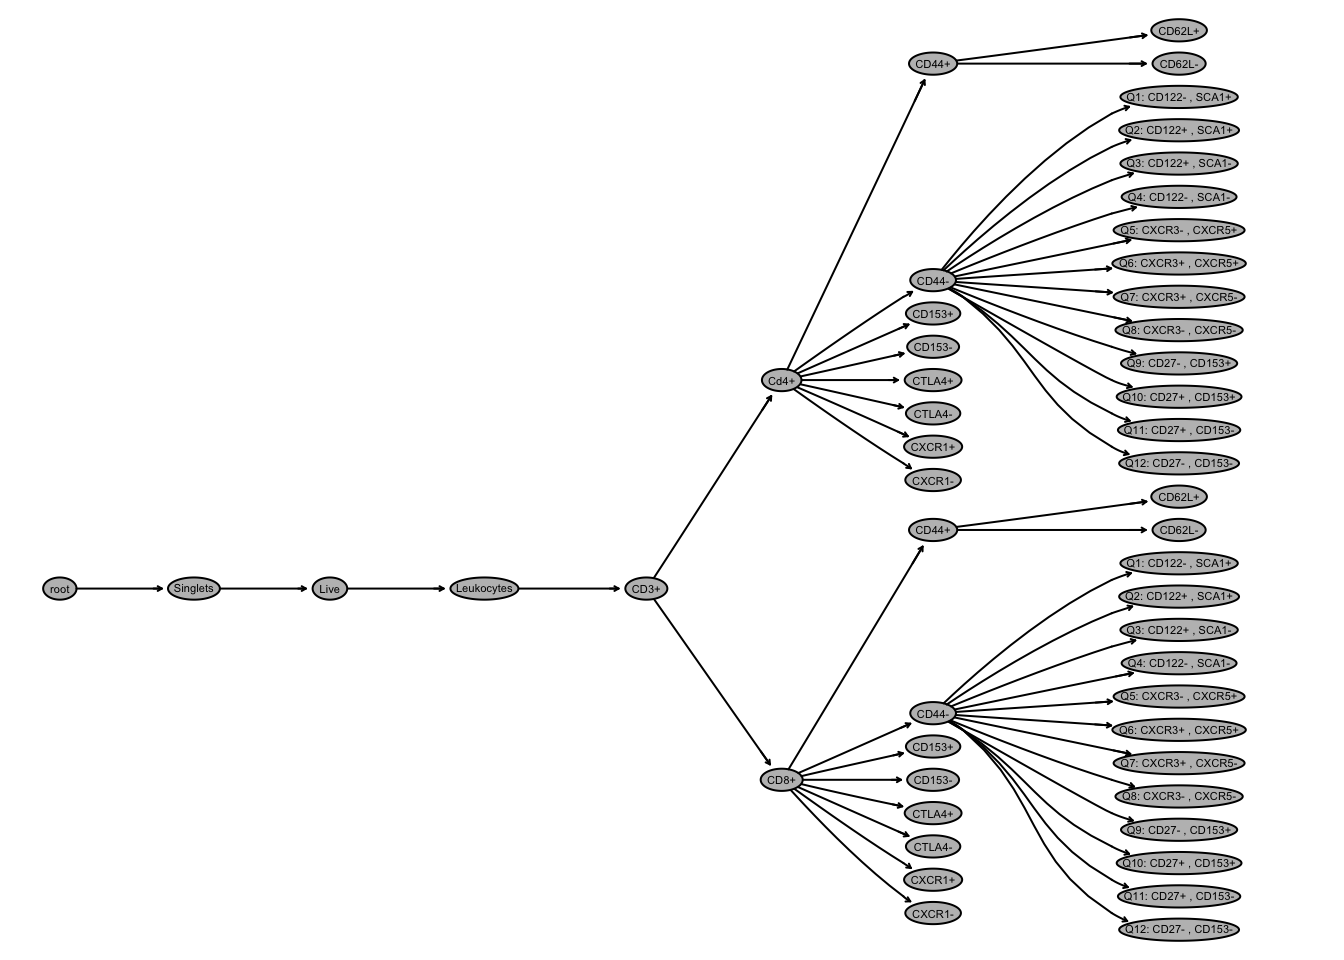
\includegraphics{bookdown_autogating_files/figure-latex/manual hierarchy-1.pdf}

\hypertarget{plotgate}{%
\subsection{plotGate()}\label{plotgate}}

The plotGate() function will gate the designated subset of your data according to parameters replicated from flowJo.

\begin{Shaded}
\begin{Highlighting}[]
\KeywordTok{flowWorkspace.par.set}\NormalTok{(}\StringTok{"plotGate"}\NormalTok{, }\KeywordTok{list}\NormalTok{(}\DataTypeTok{xlim =} \StringTok{"data"}\NormalTok{,}
                                       \DataTypeTok{ylim =} \StringTok{"data"}\NormalTok{))}
\KeywordTok{plotGate}\NormalTok{(gh)}
\end{Highlighting}
\end{Shaded}

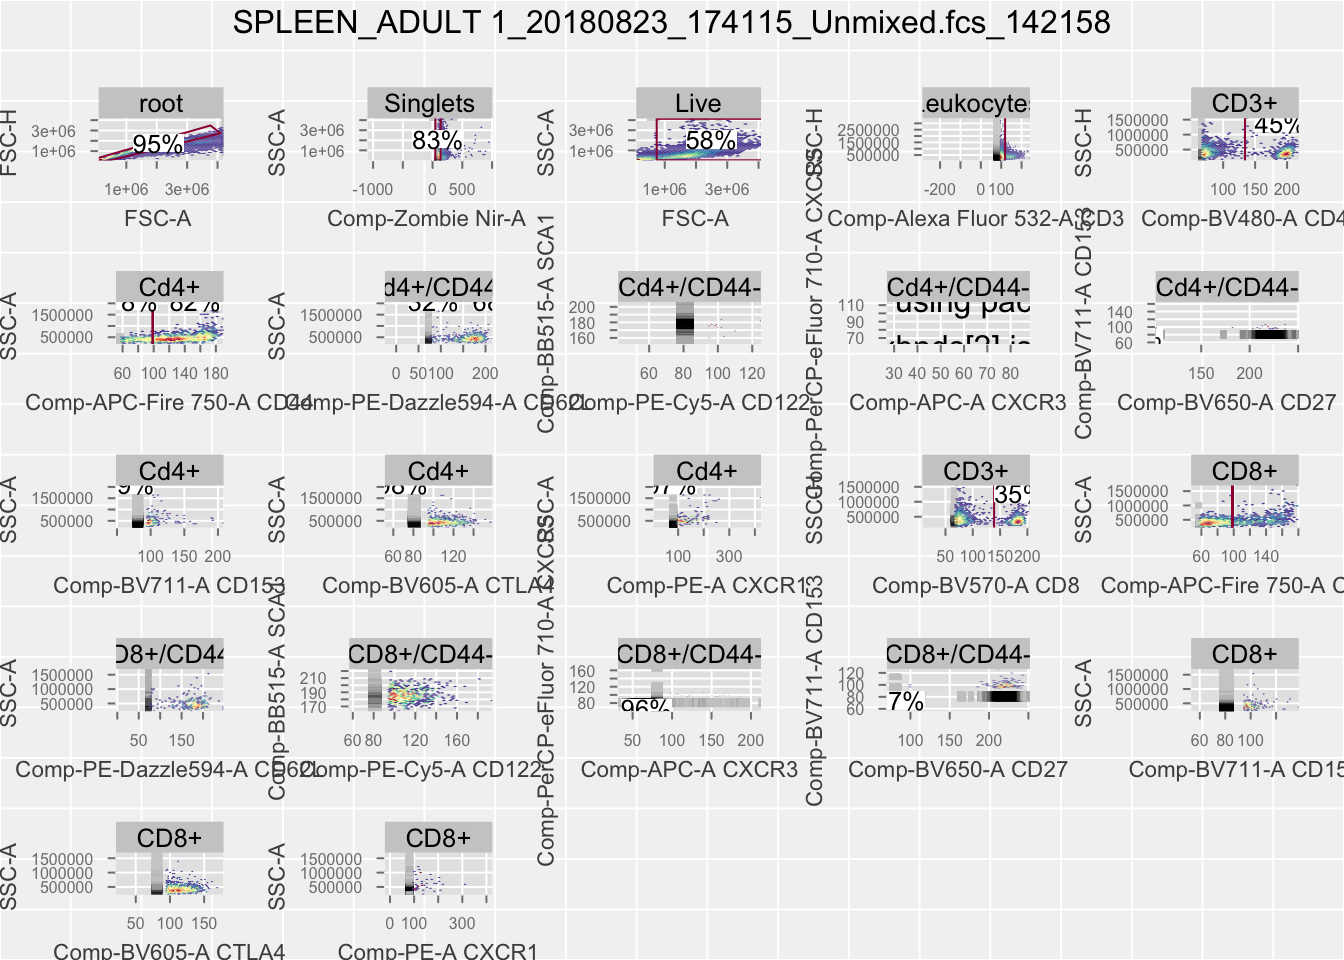
\includegraphics{bookdown_autogating_files/figure-latex/visualize subset-1.pdf}

**Note the use of \texttt{flowWorkspace.par.set()} here. Chapter 5 of this tutorial will discuss customizations such as this one.

\hypertarget{clone}{%
\section{Clone}\label{clone}}

Now, the manual gating scheme has been replicated in R using \texttt{openCyto} and verified for consistency with the original flowJo workspace. The final step in this chapter will clone \textbf{gating\_set} into a new R object named \textbf{auto\_gating}.

\begin{Shaded}
\begin{Highlighting}[]
\NormalTok{auto_gating <-}\StringTok{ }\KeywordTok{clone}\NormalTok{(gating_set)}
\KeywordTok{print}\NormalTok{(auto_gating)}
\end{Highlighting}
\end{Shaded}

\begin{verbatim}
## A GatingSet with 10 samples
\end{verbatim}

\hypertarget{create-.csv}{%
\chapter{Create .csv}\label{create-.csv}}

The creation of a .csv gating template is arguably the most important step to automating flow cytometry analysis. The .csv template that you create will tell \texttt{openCyto} how to gate your data. Gating methods that are support currently by \texttt{openCyto} include:

\emph{quadrantGate\\
}rangeGate\\
\emph{quantileGate\\
}mindensity\\
\emph{tailgate\\
}cytokine\\
\emph{flowClust\\
}boundary\\
\emph{singletGate\\
}transitional\\
\emph{plolyfunctionalityGate\\
}flowDensity

\hypertarget{csv-gating-template-structure}{%
\section{.csv Gating Template Structure}\label{csv-gating-template-structure}}

In the gating template, each row corresponds to a single cell population and the method used to gate that population. The .csv must contain 10 predefined columns that will be listed below. Most cell population names listed in columns must be uniquely and follow certain guidelines. These include:

\emph{unique idenitifer for \texttt{alias} and \texttt{parent} columns\\
}no commas in \texttt{parent} columns (otherwise \texttt{opencyto} will assume the population has multiple parents)\\
*restrict \texttt{pop} column to quadrant-only strings (++,+)

The required 10 columns are below.

\hypertarget{template-columns}{%
\subsection{Template Columns}\label{template-columns}}

\texttt{alias}- unique name/identifier for cell population\\
\texttt{pop}- +/- pattern to determine which subset or quadrant will be gated\\
\texttt{parent}- unique identifier for the parent population\\
\texttt{dims}- channel or marker names for gating\\
\texttt{gating\_method}- gating function (supported options listed above)\\
\texttt{gating\_args}- arguments to be passed to gating function
\texttt{collapseDataforGating}- data is collapsed and replicated across all samples\\
\texttt{groupBy}- used to group samples into unique combinations\\
\texttt{preprocessing\_method}- preprocessing function\\
\texttt{preprocessing\_args}- arguments for preprocessing function

\hypertarget{creating-the-template}{%
\section{Creating the Template}\label{creating-the-template}}

The gating template can be created manually or assisted by the use of the \texttt{templateGen()} function. \texttt{TemplateGen()} will auto-fill the \texttt{alias}, \texttt{pop}, \texttt{parent}, and \texttt{dims} columns and the rest must be completed manually. To use \texttt{templateGen()}, you must input a GatingHierarchy object. In this example, that is \textbf{gh}, the subset created from \textbf{gating\_set}.

\begin{Shaded}
\begin{Highlighting}[]
\NormalTok{gt <-}\StringTok{ }\KeywordTok{templateGen}\NormalTok{(gh)}
\KeywordTok{print}\NormalTok{(gt)}
\end{Highlighting}
\end{Shaded}

\begin{verbatim}
##                  alias                 pop
## 1             Singlets            Singlets
## 2                 Live                Live
## 3           Leukocytes          Leukocytes
## 4                 CD3+                CD3+
## 5                 CD8+                CD8+
## 6               CXCR1-              CXCR1-
## 7               CXCR1+              CXCR1+
## 8               CTLA4-              CTLA4-
## 9               CTLA4+              CTLA4+
## 10              CD153-              CD153-
## 11              CD153+              CD153+
## 12               CD44-               CD44-
## 13 Q12: CD27- , CD153- Q12: CD27- , CD153-
## 14 Q11: CD27+ , CD153- Q11: CD27+ , CD153-
## 15 Q10: CD27+ , CD153+ Q10: CD27+ , CD153+
## 16  Q9: CD27- , CD153+  Q9: CD27- , CD153+
## 17 Q8: CXCR3- , CXCR5- Q8: CXCR3- , CXCR5-
## 18 Q7: CXCR3+ , CXCR5- Q7: CXCR3+ , CXCR5-
## 19 Q6: CXCR3+ , CXCR5+ Q6: CXCR3+ , CXCR5+
## 20 Q5: CXCR3- , CXCR5+ Q5: CXCR3- , CXCR5+
## 21  Q4: CD122- , SCA1-  Q4: CD122- , SCA1-
## 22  Q3: CD122+ , SCA1-  Q3: CD122+ , SCA1-
## 23  Q2: CD122+ , SCA1+  Q2: CD122+ , SCA1+
## 24  Q1: CD122- , SCA1+  Q1: CD122- , SCA1+
## 25               CD44+               CD44+
## 26              CD62L-              CD62L-
## 27              CD62L+              CD62L+
## 28                Cd4+                Cd4+
## 29              CXCR1-              CXCR1-
## 30              CXCR1+              CXCR1+
## 31              CTLA4-              CTLA4-
## 32              CTLA4+              CTLA4+
## 33              CD153-              CD153-
## 34              CD153+              CD153+
## 35               CD44-               CD44-
## 36 Q12: CD27- , CD153- Q12: CD27- , CD153-
## 37 Q11: CD27+ , CD153- Q11: CD27+ , CD153-
## 38 Q10: CD27+ , CD153+ Q10: CD27+ , CD153+
## 39  Q9: CD27- , CD153+  Q9: CD27- , CD153+
## 40 Q8: CXCR3- , CXCR5- Q8: CXCR3- , CXCR5-
## 41 Q7: CXCR3+ , CXCR5- Q7: CXCR3+ , CXCR5-
## 42 Q6: CXCR3+ , CXCR5+ Q6: CXCR3+ , CXCR5+
## 43 Q5: CXCR3- , CXCR5+ Q5: CXCR3- , CXCR5+
## 44  Q4: CD122- , SCA1-  Q4: CD122- , SCA1-
## 45  Q3: CD122+ , SCA1-  Q3: CD122+ , SCA1-
## 46  Q2: CD122+ , SCA1+  Q2: CD122+ , SCA1+
## 47  Q1: CD122- , SCA1+  Q1: CD122- , SCA1+
## 48               CD44+               CD44+
## 49              CD62L-              CD62L-
## 50              CD62L+              CD62L+
##                                       parent
## 1                                       root
## 2                                  /Singlets
## 3                             /Singlets/Live
## 4                  /Singlets/Live/Leukocytes
## 5             /Singlets/Live/Leukocytes/CD3+
## 6        /Singlets/Live/Leukocytes/CD3+/CD8+
## 7        /Singlets/Live/Leukocytes/CD3+/CD8+
## 8        /Singlets/Live/Leukocytes/CD3+/CD8+
## 9        /Singlets/Live/Leukocytes/CD3+/CD8+
## 10       /Singlets/Live/Leukocytes/CD3+/CD8+
## 11       /Singlets/Live/Leukocytes/CD3+/CD8+
## 12       /Singlets/Live/Leukocytes/CD3+/CD8+
## 13 /Singlets/Live/Leukocytes/CD3+/CD8+/CD44-
## 14 /Singlets/Live/Leukocytes/CD3+/CD8+/CD44-
## 15 /Singlets/Live/Leukocytes/CD3+/CD8+/CD44-
## 16 /Singlets/Live/Leukocytes/CD3+/CD8+/CD44-
## 17 /Singlets/Live/Leukocytes/CD3+/CD8+/CD44-
## 18 /Singlets/Live/Leukocytes/CD3+/CD8+/CD44-
## 19 /Singlets/Live/Leukocytes/CD3+/CD8+/CD44-
## 20 /Singlets/Live/Leukocytes/CD3+/CD8+/CD44-
## 21 /Singlets/Live/Leukocytes/CD3+/CD8+/CD44-
## 22 /Singlets/Live/Leukocytes/CD3+/CD8+/CD44-
## 23 /Singlets/Live/Leukocytes/CD3+/CD8+/CD44-
## 24 /Singlets/Live/Leukocytes/CD3+/CD8+/CD44-
## 25       /Singlets/Live/Leukocytes/CD3+/CD8+
## 26 /Singlets/Live/Leukocytes/CD3+/CD8+/CD44+
## 27 /Singlets/Live/Leukocytes/CD3+/CD8+/CD44+
## 28            /Singlets/Live/Leukocytes/CD3+
## 29       /Singlets/Live/Leukocytes/CD3+/Cd4+
## 30       /Singlets/Live/Leukocytes/CD3+/Cd4+
## 31       /Singlets/Live/Leukocytes/CD3+/Cd4+
## 32       /Singlets/Live/Leukocytes/CD3+/Cd4+
## 33       /Singlets/Live/Leukocytes/CD3+/Cd4+
## 34       /Singlets/Live/Leukocytes/CD3+/Cd4+
## 35       /Singlets/Live/Leukocytes/CD3+/Cd4+
## 36 /Singlets/Live/Leukocytes/CD3+/Cd4+/CD44-
## 37 /Singlets/Live/Leukocytes/CD3+/Cd4+/CD44-
## 38 /Singlets/Live/Leukocytes/CD3+/Cd4+/CD44-
## 39 /Singlets/Live/Leukocytes/CD3+/Cd4+/CD44-
## 40 /Singlets/Live/Leukocytes/CD3+/Cd4+/CD44-
## 41 /Singlets/Live/Leukocytes/CD3+/Cd4+/CD44-
## 42 /Singlets/Live/Leukocytes/CD3+/Cd4+/CD44-
## 43 /Singlets/Live/Leukocytes/CD3+/Cd4+/CD44-
## 44 /Singlets/Live/Leukocytes/CD3+/Cd4+/CD44-
## 45 /Singlets/Live/Leukocytes/CD3+/Cd4+/CD44-
## 46 /Singlets/Live/Leukocytes/CD3+/Cd4+/CD44-
## 47 /Singlets/Live/Leukocytes/CD3+/Cd4+/CD44-
## 48       /Singlets/Live/Leukocytes/CD3+/Cd4+
## 49 /Singlets/Live/Leukocytes/CD3+/Cd4+/CD44+
## 50 /Singlets/Live/Leukocytes/CD3+/Cd4+/CD44+
##                                  dims gating_method gating_args
## 1                         FSC-A,FSC-H          <NA>        <NA>
## 2                   Comp-Zombie Nir-A          <NA>        <NA>
## 3                         FSC-A,SSC-A          <NA>        <NA>
## 4        Comp-Alexa Fluor 532-A,SSC-H          <NA>        <NA>
## 5                  Comp-BV570-A,SSC-H          <NA>        <NA>
## 6                           Comp-PE-A          <NA>        <NA>
## 7                           Comp-PE-A          <NA>        <NA>
## 8                        Comp-BV605-A          <NA>        <NA>
## 9                        Comp-BV605-A          <NA>        <NA>
## 10                       Comp-BV711-A          <NA>        <NA>
## 11                       Comp-BV711-A          <NA>        <NA>
## 12                Comp-APC-Fire 750-A          <NA>        <NA>
## 13          Comp-BV650-A,Comp-BV711-A          <NA>        <NA>
## 14          Comp-BV650-A,Comp-BV711-A          <NA>        <NA>
## 15          Comp-BV650-A,Comp-BV711-A          <NA>        <NA>
## 16          Comp-BV650-A,Comp-BV711-A          <NA>        <NA>
## 17 Comp-APC-A,Comp-PerCP-eFluor 710-A          <NA>        <NA>
## 18 Comp-APC-A,Comp-PerCP-eFluor 710-A          <NA>        <NA>
## 19 Comp-APC-A,Comp-PerCP-eFluor 710-A          <NA>        <NA>
## 20 Comp-APC-A,Comp-PerCP-eFluor 710-A          <NA>        <NA>
## 21         Comp-PE-Cy5-A,Comp-BB515-A          <NA>        <NA>
## 22         Comp-PE-Cy5-A,Comp-BB515-A          <NA>        <NA>
## 23         Comp-PE-Cy5-A,Comp-BB515-A          <NA>        <NA>
## 24         Comp-PE-Cy5-A,Comp-BB515-A          <NA>        <NA>
## 25                Comp-APC-Fire 750-A          <NA>        <NA>
## 26                Comp-PE-Dazzle594-A          <NA>        <NA>
## 27                Comp-PE-Dazzle594-A          <NA>        <NA>
## 28                 Comp-BV480-A,SSC-H          <NA>        <NA>
## 29                          Comp-PE-A          <NA>        <NA>
## 30                          Comp-PE-A          <NA>        <NA>
## 31                       Comp-BV605-A          <NA>        <NA>
## 32                       Comp-BV605-A          <NA>        <NA>
## 33                       Comp-BV711-A          <NA>        <NA>
## 34                       Comp-BV711-A          <NA>        <NA>
## 35                Comp-APC-Fire 750-A          <NA>        <NA>
## 36          Comp-BV650-A,Comp-BV711-A          <NA>        <NA>
## 37          Comp-BV650-A,Comp-BV711-A          <NA>        <NA>
## 38          Comp-BV650-A,Comp-BV711-A          <NA>        <NA>
## 39          Comp-BV650-A,Comp-BV711-A          <NA>        <NA>
## 40 Comp-APC-A,Comp-PerCP-eFluor 710-A          <NA>        <NA>
## 41 Comp-APC-A,Comp-PerCP-eFluor 710-A          <NA>        <NA>
## 42 Comp-APC-A,Comp-PerCP-eFluor 710-A          <NA>        <NA>
## 43 Comp-APC-A,Comp-PerCP-eFluor 710-A          <NA>        <NA>
## 44         Comp-PE-Cy5-A,Comp-BB515-A          <NA>        <NA>
## 45         Comp-PE-Cy5-A,Comp-BB515-A          <NA>        <NA>
## 46         Comp-PE-Cy5-A,Comp-BB515-A          <NA>        <NA>
## 47         Comp-PE-Cy5-A,Comp-BB515-A          <NA>        <NA>
## 48                Comp-APC-Fire 750-A          <NA>        <NA>
## 49                Comp-PE-Dazzle594-A          <NA>        <NA>
## 50                Comp-PE-Dazzle594-A          <NA>        <NA>
##    collapseDataForGating groupBy preprocessing_method preprocessing_args
## 1                   <NA>    <NA>                 <NA>               <NA>
## 2                   <NA>    <NA>                 <NA>               <NA>
## 3                   <NA>    <NA>                 <NA>               <NA>
## 4                   <NA>    <NA>                 <NA>               <NA>
## 5                   <NA>    <NA>                 <NA>               <NA>
## 6                   <NA>    <NA>                 <NA>               <NA>
## 7                   <NA>    <NA>                 <NA>               <NA>
## 8                   <NA>    <NA>                 <NA>               <NA>
## 9                   <NA>    <NA>                 <NA>               <NA>
## 10                  <NA>    <NA>                 <NA>               <NA>
## 11                  <NA>    <NA>                 <NA>               <NA>
## 12                  <NA>    <NA>                 <NA>               <NA>
## 13                  <NA>    <NA>                 <NA>               <NA>
## 14                  <NA>    <NA>                 <NA>               <NA>
## 15                  <NA>    <NA>                 <NA>               <NA>
## 16                  <NA>    <NA>                 <NA>               <NA>
## 17                  <NA>    <NA>                 <NA>               <NA>
## 18                  <NA>    <NA>                 <NA>               <NA>
## 19                  <NA>    <NA>                 <NA>               <NA>
## 20                  <NA>    <NA>                 <NA>               <NA>
## 21                  <NA>    <NA>                 <NA>               <NA>
## 22                  <NA>    <NA>                 <NA>               <NA>
## 23                  <NA>    <NA>                 <NA>               <NA>
## 24                  <NA>    <NA>                 <NA>               <NA>
## 25                  <NA>    <NA>                 <NA>               <NA>
## 26                  <NA>    <NA>                 <NA>               <NA>
## 27                  <NA>    <NA>                 <NA>               <NA>
## 28                  <NA>    <NA>                 <NA>               <NA>
## 29                  <NA>    <NA>                 <NA>               <NA>
## 30                  <NA>    <NA>                 <NA>               <NA>
## 31                  <NA>    <NA>                 <NA>               <NA>
## 32                  <NA>    <NA>                 <NA>               <NA>
## 33                  <NA>    <NA>                 <NA>               <NA>
## 34                  <NA>    <NA>                 <NA>               <NA>
## 35                  <NA>    <NA>                 <NA>               <NA>
## 36                  <NA>    <NA>                 <NA>               <NA>
## 37                  <NA>    <NA>                 <NA>               <NA>
## 38                  <NA>    <NA>                 <NA>               <NA>
## 39                  <NA>    <NA>                 <NA>               <NA>
## 40                  <NA>    <NA>                 <NA>               <NA>
## 41                  <NA>    <NA>                 <NA>               <NA>
## 42                  <NA>    <NA>                 <NA>               <NA>
## 43                  <NA>    <NA>                 <NA>               <NA>
## 44                  <NA>    <NA>                 <NA>               <NA>
## 45                  <NA>    <NA>                 <NA>               <NA>
## 46                  <NA>    <NA>                 <NA>               <NA>
## 47                  <NA>    <NA>                 <NA>               <NA>
## 48                  <NA>    <NA>                 <NA>               <NA>
## 49                  <NA>    <NA>                 <NA>               <NA>
## 50                  <NA>    <NA>                 <NA>               <NA>
\end{verbatim}

The auto-filled template will generate within the R Console and can then be saved locally with the following code.

\begin{Shaded}
\begin{Highlighting}[]
\KeywordTok{write.csv}\NormalTok{(gt, }\StringTok{"gt.csv"}\NormalTok{)}
\end{Highlighting}
\end{Shaded}

If you choose to create the gating template manually, the same conventions must be followed. Start with a blank spreadsheet. Next, fill in the 10 required column names. From there, use the manual gating hierarchy to fill in each cell population \texttt{alias}. Fill in the remainder accordingly.

There will likely be troubleshooting involved in this process. \href{https://www.bioconductor.org/packages/devel/bioc/vignettes/openCyto/inst/doc/HowToWriteCSVTemplate.html\#14_gating_method_that_generates_multiple_populations}{This} is a great place to start if you're seeking more information on the gating template.

\hypertarget{load-.csv-into-r}{%
\section{Load .csv into R}\label{load-.csv-into-r}}

When the .csv gating template is complete, it is then read into R and saved as \textbf{gt}. The gating template will be saved as a GatingTemplate object.

\begin{Shaded}
\begin{Highlighting}[]
\NormalTok{gt <-}\StringTok{ }\KeywordTok{gatingTemplate}\NormalTok{(}\StringTok{"/Users/monhait/Desktop/flow_cyto/automated_gating/data/gating_template/auto_template_1.csv"}\NormalTok{,}
                     \DataTypeTok{strict =} \OtherTok{FALSE}\NormalTok{, }\DataTypeTok{strip_extra_quotes =} \OtherTok{TRUE}\NormalTok{)}
\KeywordTok{print}\NormalTok{(gt)}
\end{Highlighting}
\end{Shaded}

\hypertarget{automate-gating}{%
\chapter{Automate Gating}\label{automate-gating}}

The flow cytometry equipment at CSU will compensate and transform the data automatically. Other tutorials may highlight the steps to compensate and transform data, but these are not relevant to CSU at this moment. In the event that equipment changes, it may be necessary to complete compensation and transformation steps to prepare data. More on the current equipment used as CSU \href{https://www.umassmed.edu/facslab/instrument/core-cytek-aurora2/}{here}.

\hypertarget{apply-gating}{%
\section{Apply Gating}\label{apply-gating}}

At this point, you will either return to your cloned GatingSet object that contains raw FCS files or bring in new data to be gated using the same parameters. Apply \textbf{gt} to the GatingSet object, where x = \textbf{gt} and y = data to be gated.

\begin{Shaded}
\begin{Highlighting}[]
\KeywordTok{gating}\NormalTok{(}\DataTypeTok{x =}\NormalTok{ gt, }\DataTypeTok{y =}\NormalTok{ auto_gating)}
\end{Highlighting}
\end{Shaded}

Just as before, plot both the gating hierarchy and the automated gates. You may notice extra nodes have been added to the hierarchy. Chapter 5 will highlight additional cusomization to remove unwanted nodes and improve upon visualization.

\hypertarget{plot-automated-gating}{%
\section{Plot Automated Gating}\label{plot-automated-gating}}

\begin{Shaded}
\begin{Highlighting}[]
\KeywordTok{plotGate}\NormalTok{(auto_gating)}
\end{Highlighting}
\end{Shaded}

\begin{Shaded}
\begin{Highlighting}[]
\KeywordTok{plot}\NormalTok{(auto_gating)}
\end{Highlighting}
\end{Shaded}

\hypertarget{population-statistics}{%
\section{Population Statistics}\label{population-statistics}}

Both counts and frequencies can be generated for analysis. This can be generate based on the analysis completed in R, or pulled directly from flowJo. To pull from flowJo, simply at \texttt{flowJo=TRUE} to either code chunk below.

\textbf{Counts}

\begin{Shaded}
\begin{Highlighting}[]
\KeywordTok{head}\NormalTok{(}\KeywordTok{getPopStats}\NormalTok{(auto_gating,}\DataTypeTok{satistic=}\StringTok{"count"}\NormalTok{))}
\end{Highlighting}
\end{Shaded}

\begin{verbatim}
##                                                 name Population     Parent
## 1: SPLEEN_ADULT 1_20180823_174115_Unmixed.fcs_142158   Singlets       root
## 2: SPLEEN_ADULT 1_20180823_174115_Unmixed.fcs_142158       Live   Singlets
## 3: SPLEEN_ADULT 1_20180823_174115_Unmixed.fcs_142158 Leukocytes       Live
## 4: SPLEEN_ADULT 1_20180823_174115_Unmixed.fcs_142158       CD3+ Leukocytes
## 5: SPLEEN_ADULT 1_20180823_174115_Unmixed.fcs_142158       Cd4+       CD3+
## 6: SPLEEN_ADULT 1_20180823_174115_Unmixed.fcs_142158 Cd4+/CD44+       Cd4+
##     Count ParentCount
## 1: 134378      142158
## 2: 111695      134378
## 3:  65104      111695
## 4:   4781       65104
## 5:   2151        4781
## 6:   1760        2151
\end{verbatim}

\textbf{Frequencies}

\begin{Shaded}
\begin{Highlighting}[]
\KeywordTok{head}\NormalTok{(}\KeywordTok{getPopStats}\NormalTok{(auto_gating,}\DataTypeTok{satistic=}\StringTok{"freq"}\NormalTok{))}
\end{Highlighting}
\end{Shaded}

\begin{verbatim}
##                                                 name Population     Parent
## 1: SPLEEN_ADULT 1_20180823_174115_Unmixed.fcs_142158   Singlets       root
## 2: SPLEEN_ADULT 1_20180823_174115_Unmixed.fcs_142158       Live   Singlets
## 3: SPLEEN_ADULT 1_20180823_174115_Unmixed.fcs_142158 Leukocytes       Live
## 4: SPLEEN_ADULT 1_20180823_174115_Unmixed.fcs_142158       CD3+ Leukocytes
## 5: SPLEEN_ADULT 1_20180823_174115_Unmixed.fcs_142158       Cd4+       CD3+
## 6: SPLEEN_ADULT 1_20180823_174115_Unmixed.fcs_142158 Cd4+/CD44+       Cd4+
##     Count ParentCount
## 1: 134378      142158
## 2: 111695      134378
## 3:  65104      111695
## 4:   4781       65104
## 5:   2151        4781
## 6:   1760        2151
\end{verbatim}

\hypertarget{customization}{%
\chapter{Customization}\label{customization}}

It is possible that additional customization may be necessary when working with the \texttt{openCyto} framework. Below are three common customizations that will be outlined in this chapter.

\begin{enumerate}
\def\labelenumi{\arabic{enumi}.}
\tightlist
\item
  Hiding unwanted nodes
\item
  Renaming nodes
\item
  Adjusting plots
\end{enumerate}

\hypertarget{hiding-unwanted-nodes}{%
\section{Hiding unwanted nodes}\label{hiding-unwanted-nodes}}

When automating analysis, there may be nodes that were not predefined in the .csv gating template or nodes that may not be of interest in your particular analysis. Plotting the gating hierarchy using the \texttt{plot()} function will display this and then nodes can be hidden based on need with the following code. Below is an example of a ``full'' gating hierarchy and then the same hierarchy with the CD3+ node removed.

\textbf{Full Hierarchy}

\begin{Shaded}
\begin{Highlighting}[]
\KeywordTok{plot}\NormalTok{(gh)}
\end{Highlighting}
\end{Shaded}

\textbf{CD3+ Removed Hierarchy}

To remove nodes, first save the unwanted nodes as an R object named \textbf{nodesToHide}. Next, use the code following the \texttt{lapply()} function, only replacing \textbf{gs} with your GatingSet object name.

\begin{Shaded}
\begin{Highlighting}[]
\NormalTok{nodesToHide <-}\StringTok{ "CD3+"}
\KeywordTok{lapply}\NormalTok{(nodesToHide, }\ControlFlowTok{function}\NormalTok{(thisNode)}\KeywordTok{setNode}\NormalTok{(gs, thisNode, }\OtherTok{FALSE}\NormalTok{))}
\end{Highlighting}
\end{Shaded}

\hypertarget{renaming-nodes}{%
\section{Renaming nodes}\label{renaming-nodes}}

Rename nodes based on your preferences with the following code. Within the \texttt{setNode} function, the first input is the current cell population name and the second is the desired change.

\begin{Shaded}
\begin{Highlighting}[]
\KeywordTok{setNode}\NormalTok{(}\StringTok{"Live"}\NormalTok{, }\StringTok{"Viable"}\NormalTok{)}
\end{Highlighting}
\end{Shaded}

\hypertarget{adjusting-plots}{%
\section{Adjusting plots}\label{adjusting-plots}}

\hypertarget{adjust-plot-axes}{%
\subsection{Adjust plot axes}\label{adjust-plot-axes}}

As seen in chapter 2, it may be necessary to adjust the plot axes in order to best view the gates. This is done using the code below. Setting xlim and ylim to ``data'' adjusts plot based on the actual data range, rather than instrument specifications. Custom ranges can also be input numerically.

\begin{Shaded}
\begin{Highlighting}[]
\KeywordTok{flowWorkspace.par.set}\NormalTok{(}\StringTok{"plotGate"}\NormalTok{, }\KeywordTok{list}\NormalTok{(}\DataTypeTok{xlim =} \StringTok{"data"}\NormalTok{,}
                                       \DataTypeTok{ylim =} \StringTok{"data"}\NormalTok{))}
\end{Highlighting}
\end{Shaded}

Here is a comparison of xlim and ylim set as ``instrument'' and then ``data''.

\textbf{Instrument}

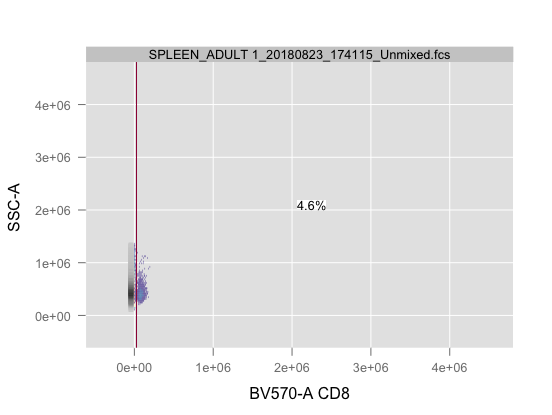
\includegraphics[width=0.6\linewidth]{/Users/monhait/Desktop/bookdown_autogating/images/CD8_instrument}

\textbf{Data}

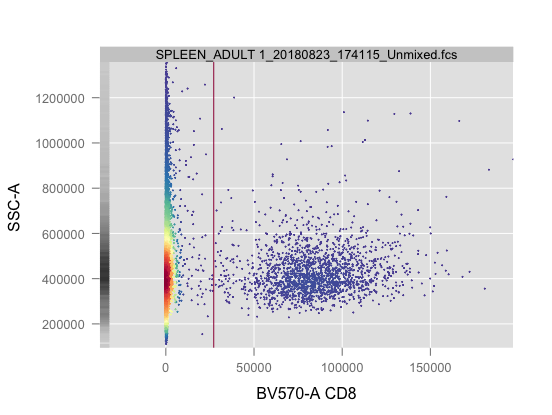
\includegraphics[width=0.6\linewidth]{/Users/monhait/Desktop/bookdown_autogating/images/cd8_data}

\hypertarget{transform-data-for-better-visualization}{%
\subsection{Transform data for better visualization}\label{transform-data-for-better-visualization}}

Although data will not be altered in any way, transformation may allow for better visualization. The most common form of transformation for flow cytometry analysis is \href{http://docs.flowjo.com/vx/graphs-and-gating/gw-transform-overview/}{bioexponential}. Below is a comparison of gates without transformation and gates that have been transformed.

\textbf{Without Transformation}

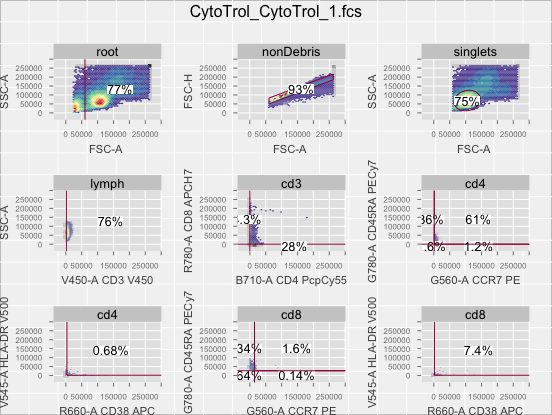
\includegraphics[width=0.6\linewidth]{/Users/monhait/Desktop/bookdown_autogating/images/no_trans}

\textbf{Transformed}

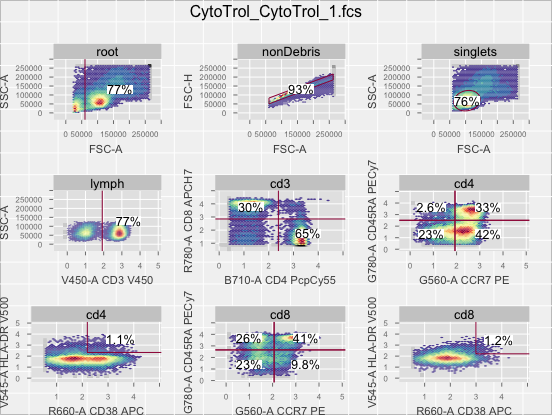
\includegraphics[width=0.6\linewidth]{/Users/monhait/Desktop/bookdown_autogating/images/trans}


\end{document}
